\chapter{Distribución del producto}

Para poder usar twinX, dado que está pensado para ser accedido desde la web, tenemos que tenerlo primeramente alojado en un servidor, de modo que pueda ser accesible desde cualquier parte y con cualquier dispositivo. Hasta ahora, el desarrollo se ha llevado a cabo en un entorno de Apache \cite{apache}, mediante la ayuda de XAMPP, y  hemos podido sistematizar el funcionamiento de un \textit{webserver}. Sin embargo, para hacer las pruebas ha sido necesario alojar twinX en un servidor, al igual que para su distribución será necesario, igualmente.

\section{Despliegue (deployment)}

Dado que Amazon oferta una licencia gratuita hasta el año de graduación para estudiantes, se ha hecho uso de la herramienta AWS \cite{aws} por ello y por su gran potencial. Nosotros tan solo necesitaremos desplegar nuestra aplicación, pero hoy por hoy resulta una de las mejores alternativas, por su amplia gama de productos y su buen funcionamiento.

Para tener nuestro sitio web alojado, tras registrarnos en AWS Educate \cite{awseducate}, lo primero que tenemos que hacer es crear una instancia de máquina virtual \textbf{EC2}. Para nuestro despliegue, hemos usado una máquina con Windows Server\textregistered 2019 Datacenter, unos 30 GB de disco duro, 1 GB de RAM y un procesador Intel(R) Xeon(R) CPU E5-2676 v3 @ 2.40 GHz con un \textit{core} físico, que es lo que nos ofrece AWS en el \textit{free tier}.

Tras la creación de la instancia, se nos proporciona una clave privada que nos permitirá conectarnos al servidor. La ventaja de haber escogido Windows Server como sistema es la posibilidad de conectarnos de forma remota desde el escritorio de un ordenador con Windows y poder interaccionar como si fuera una máquina virtual local. Una vez está todo listo, aportando el archivo con la clave privada, se descarga una conexión preparada a la máquina, y con tan solo ejecutarla e introducir la clave, ya tenemos acceso a su escritorio remoto.

Una vez conectados, hemos de cambiar las preferencias del firewall (figura \ref{fig:firewall}) para poder acceder desde otro equipo. 

\begin{figure}
	\centering
	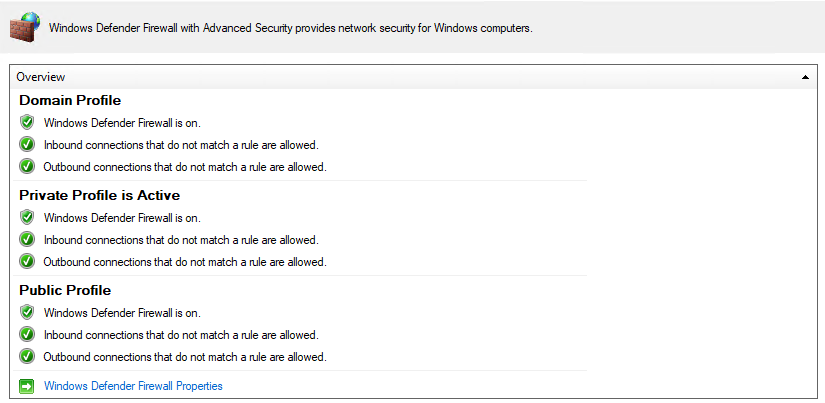
\includegraphics[width=\linewidth]{img/firewall}
	\caption{Configuración del firewall de la instancia de AWS}
	\label{fig:firewall}
\end{figure}

Es entonces cuando podemos proceder con la instalación de \textbf{WAMP} \cite{wamp}, la pila software que configuraremos del mismo modo que hemos explicado en la sección \ref{sec:herramientasdesarrollo} con XAMPP. Hay que tener especial cuidado a la hora de instalar las dependencias, puesto que son bastantes (Microsoft Visual C++ en sus numerosas versiones).

Con todo instalado, podemos observar que WAMP corre en segundo plano en la barra de estado del sistema (figura \ref{fig:wamp}). Una vez hemos modificado el archivo \\ \texttt{httpd-vhosts.conf} de Apache para aceptar todas las conexiones externas con la regla \texttt{Require all granted}, podemos establecer desde nuestro sistema la conexión con el servidor, y veremos la pantalla de la figura \ref{fig:wampinit}.

\begin{figure}
	\centering
	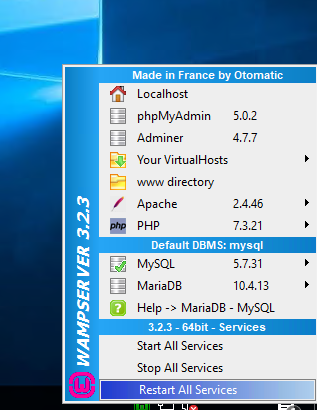
\includegraphics{img/wamp}
	\caption{Estado de WAMP}
	\label{fig:wamp}
\end{figure}

\begin{figure}
	\centering
	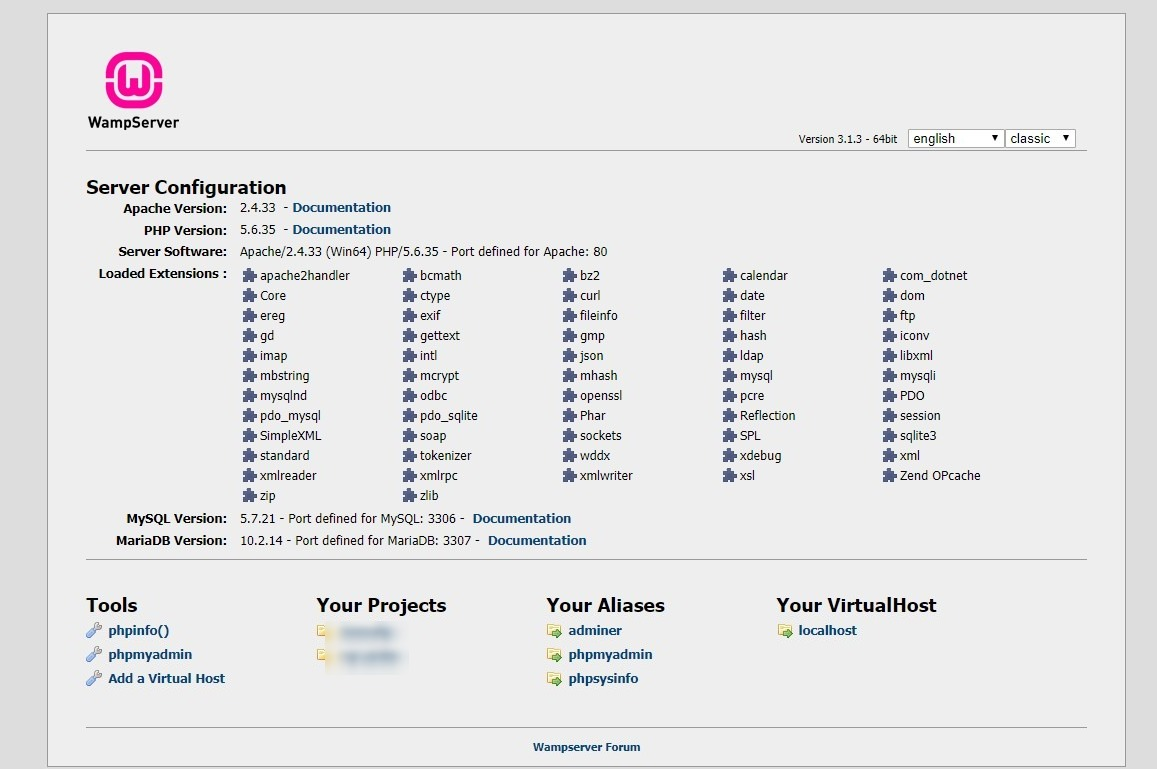
\includegraphics[width=\linewidth]{img/wampinit}
	\caption[Página principal de WAMP]{Página principal de WAMP (recuperado de: https://phantomthemes.com/wp-content/uploads/2018/06/wampserver-default-localhost-page1.jpg)}
	\label{fig:wampinit}
\end{figure}

Es entonces cuando podemos proceder a transferir los archivos del proyecto de twinX al servidor. De nuevo, gracias a la conexión con el escritorio remoto, esto es posible de hacer con tan solo arrastrar dentro del servidor los archivos. 

Una vez en el servidor, lo siguiente fue la instalación de GitHub Desktop \cite{githubdesktop} en el servidor. Si bien ya lo veníamos utilizando para hacer las copias de seguridad del proyecto durante todo su desarrollo, ahora vamos a aprovecharnos de la comodidad que supone el hacer un \textit{commit} en el equipo local y poder conectarnos de forma remota para actualizar el repositorio y que la versión desplegada en el servidor se renueve a la par. No obstante, para la primera recuperación de los archivos de la nube, la transferencia se hizo directamente desde el equipo local, dado que no se salvaguarda la carpeta \texttt{vendor}, entre otras, donde se tiene el núcleo de Yii2 y las dependencias de librerías que hemos necesitado instalar para llevar a cabo el desarrollo de twinX.

Antes de comenzar a usar Composer en el servidor para instalar las dependencias necesarias, fue necesario ajustar la versión de PHP en el servidor. Parece cosa fácil si se hace desde el menu de WAMP, pero en el fondo no se está cambiando más que la versión que ejecuta el sistema al interpretar el código que se sirve, pero no la del intérprete de la línea de comandos (\texttt{CLI}). Para conseguir esto, fue necesario ajustar que Composer hiciera uso del ejecutable de la versión 7.3.21, cambiando el directorio de PHP en el \texttt{composer.bat} que se ejecuta cada vez que introducimos la orden \texttt{composer} en el CLI.

Una vez hechos los ajustes necesarios, transferido los archivos y haberlos localizado en el repositorio correspondiente (carpeta \texttt{www} del directorio de WAMP), hemos de ejecutar, el archivo \texttt{php.ini} para iniciar el entorno de producción, que difiere en el de desarrollo (utilizado hasta ahora en el equipo local durante la construcción de twinX) en la ocultación de las herramientas del desarrollador (figura \ref{fig:herramientasdesarrollo}).

\begin{figure}
	\centering
	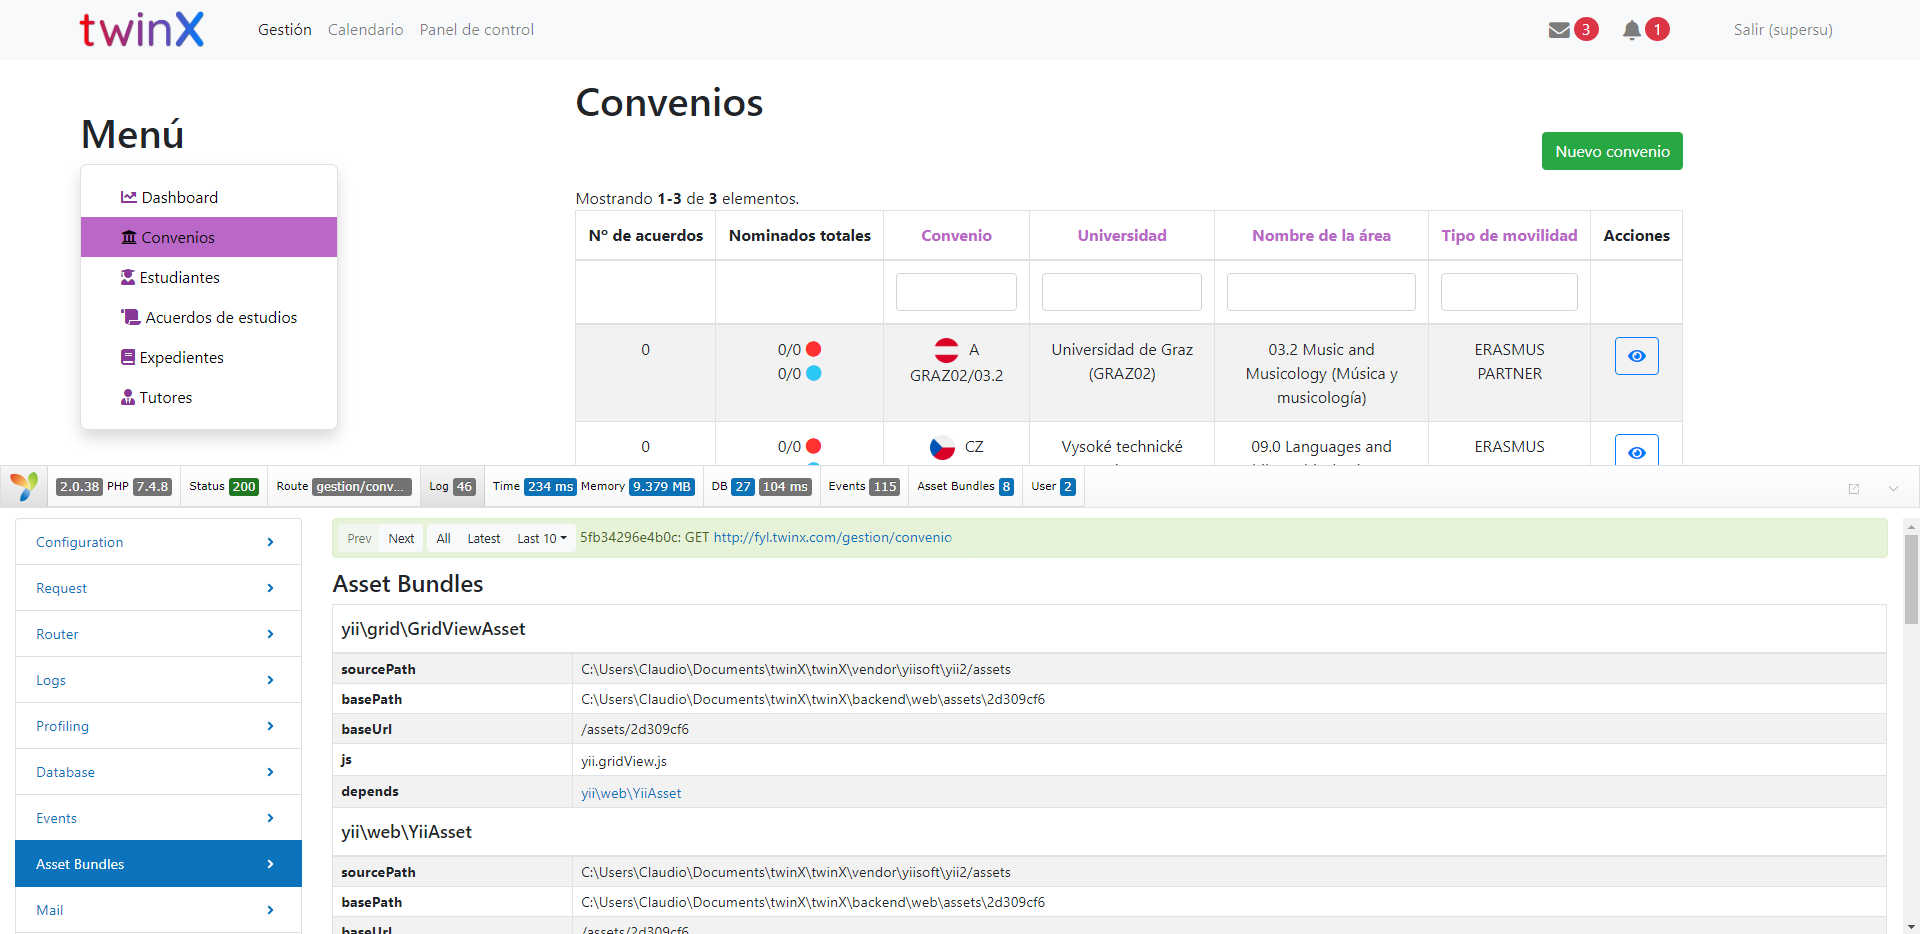
\includegraphics[width=\linewidth]{img/herramientas_desarrollo}
	\caption{Herramientas de desarrollo de Yii}
	\label{fig:herramientasdesarrollo}
\end{figure}

El siguiente paso es el de exportar la base de datos del equipo local e importarla en el servidor. Para ello, phpMyAdmin nos lo pone fácil con su herramienta de exportación. Una vez en el servidor, solo tenemos que pegar el código MySQL generado y todas las tablas con sus atributos y restricciones y las tuplas guardadas estarán disponibles en el servidor para poder trabajar con twinX.

Como resultado, estableciendo conexión al servidor con la dirección pública \cite{twinx}, podemos ver twinX en la web (figura \ref{fig:twinx}), accesible desde un navegador y con todo su funcionamiento (aunque, como es lógico, con mayor tiempo de respuesta que si se ejecutara en el mismo equipo).

\begin{figure}
	\centering
	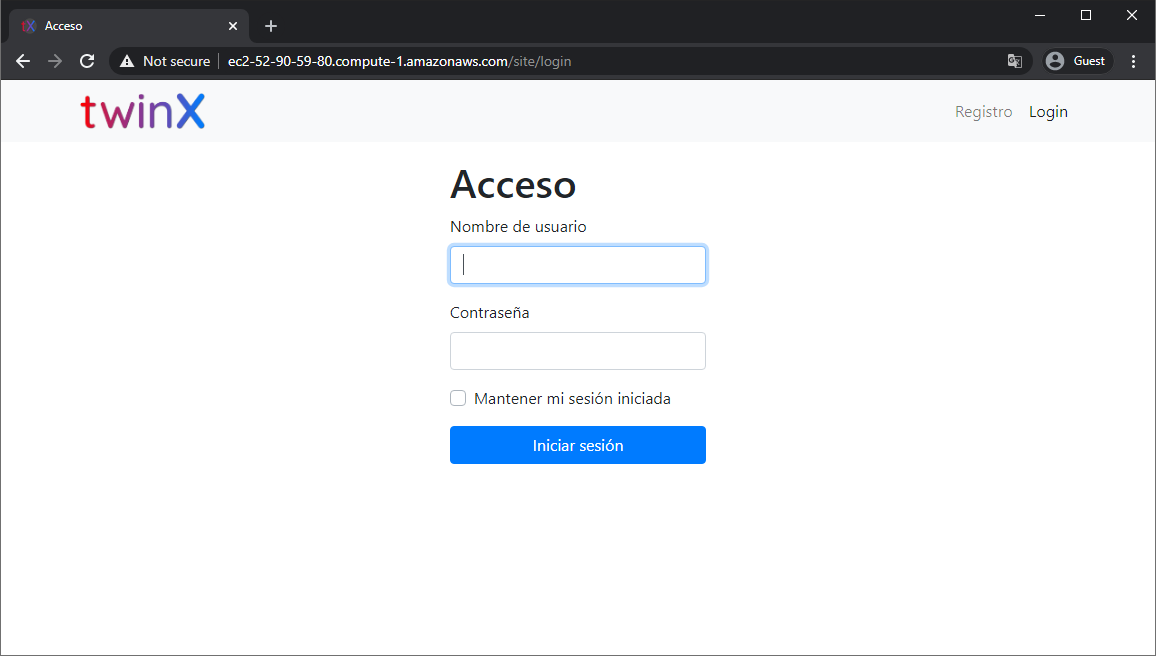
\includegraphics[width=\linewidth]{img/twinx_desplegado}
	\caption{Visualización de twinX en el servidor}
	\label{fig:twinx}
\end{figure}

